\documentclass[11pt]{aghdpl}
% \documentclass[en,11pt]{aghdpl}  % praca w języku angielskim
\usepackage[polish]{babel}
%\usepackage[english]{babel}
\usepackage[utf8]{inputenc}

% dodatkowe pakiety
\usepackage{enumerate}
\usepackage{listings}
\lstloadlanguages{TeX}

\lstset{
  literate={ą}{{\k{a}}}1
           {ć}{{\'c}}1
           {ę}{{\k{e}}}1
           {ó}{{\'o}}1
           {ń}{{\'n}}1
           {ł}{{\l{}}}1
           {ś}{{\'s}}1
           {ź}{{\'z}}1
           {ż}{{\.z}}1
           {Ą}{{\k{A}}}1
           {Ć}{{\'C}}1
           {Ę}{{\k{E}}}1
           {Ó}{{\'O}}1
           {Ń}{{\'N}}1
           {Ł}{{\L{}}}1
           {Ś}{{\'S}}1
           {Ź}{{\'Z}}1
           {Ż}{{\.Z}}1
}

%---------------------------------------------------------------------------

\author{Marcin Krupa}
\shortauthor{M. Krupa}

\titlePL{Wspieranie zespołowej analizy danych o charakterze grafowym}
\titleEN{Supporting team analysis of graph data}

\shorttitlePL{Wspieranie zespołowej analizy danych o charakterze grafowym} % skrócona wersja tytułu jeśli jest bardzo długi
\shorttitleEN{Supporting team analysis of graph data}

\thesistype{Praca dyplomowa magisterska}
%\thesistype{Master of Science Thesis}

\supervisor{dr inż. Jacek Dajda}
%\supervisor{Jacek Dajda PhD, DSc}

\degreeprogramme{Informatyka}
%\degreeprogramme{Computer Science}

\date{2013}

\department{Katedra Informatyki}
%\department{Department of Computer Science}

\faculty{Wydział Informatyki,\protect\\[-1mm] Elektroniki i Telekomunikacji}
%\faculty{Faculty of Computer Science, Electronics and Telecommunications}

\acknowledgements{Serdecznie dziękuję \dots tu ciąg dalszych podziękowań np. dla promotora, żony, sąsiada itp.}


\setlength{\cftsecnumwidth}{10mm}

%---------------------------------------------------------------------------

\begin{document}

\titlepages

\tableofcontents
\clearpage

\chapter{Wstęp}
\label{cha:wstep}


%---------------------------------------------------------------------------

\section{Cele pracy}
\label{sec:celePracy}

Celem poniższej pracy jest zaprojektowanie i stworzenie systemu kontroli wersji grafowych baz danych, będącego narzędziem wspomagającym zespołową analizę danych o charakterze grafowym.


%---------------------------------------------------------------------------

\section{Zawartość pracy}
\label{sec:zawartoscPracy}

W rodziale~\ref{cha:wprowadzenie} przedstawiono podstawowe informacje dotyczące baz NoSQL, grafowego modelu danych i systemów kontroli wersji, a także porównano dostępne na rynku grafowe bazy danych.


















\chapter{Wprowadzenie}
\label{cha:wprowadzenie}

W rozdziale tym przedstawiono podstawowe informacje dotyczące baz \emph{NoSQL} z naciskiem na bazy grafowe oraz wersjonowania danych. Porównano także dostępne na rynku rozwiązania.

%---------------------------------------------------------------------------



\section{Relacyjne bazy danych}
\label{sec:relacyjneBazyDanych}

W czerwcu 1970 Edgar Frank Codd, pracując dla IBM, opublikował ,,A Relational Model of Data for Large Shared Data Bank'' -- pracę na temat relacyjnego modelu organizacji danych. Model relacyjny i pierwowzór języka SQL po raz pierwszy zostały zaimplementowany przez IBM w projekcie System R (System Rational), będącym protoplastą DB2, prowadzonym w latach 1974–1978. Pierwsze komercyjne rozwiązania to Oracle (1979) i DB2 (1983). Relacyjne bazy danych wkrótce zawładnęły rynkiem i mimo upływu czasu, nadal są dominującą technologią, zwłaszcza wśród aplikacji biznesowych. W ciągu ponad 30 lat dominacji, co jest ewenementem w świecie informatyki, kilkukrotnie pojawiały się technologie bazodanowe z potencjałem do odebrania części rynku systemom relacyjnym, na przykład obiektowe bazy danych w latach 90'. Alternatywy te nigdy jednak nie stały sie popularne. Może więc dziwić panujące od niedawna poruszenie wokół technologii \emph{NoSQL}.

\subsection{Model relacyjny}
\label{sec:modelRelacyjny}

tu opis modelu, diagram obiektowy i erd

\subsection{Zalety relacyjnych baz danych}
\label{sec:zaletyRelacyjnychBazDanych}

Najbardziej oczywistym zastosowaniem bazy danych jest przechowywanie dużych ilości danych. Pamięć współczesnych systemów komputerowych dzieli się na szybką, ulotną pamięć operacyjną oraz wolniejszą, lecz pojemniejszą pamięć dyskową. Rozmiar pamięci operacyjnej jest ograniczony (z powodu kosztów), a dane są tracone po odłączeniu zasilania -- trwałe przechowywanie danych wymaga więc wykorzystania przestrzeni dyskowej.
Dla wielu aplikacji wystarczające jest przechowywanie danych w plikach na dysku, jednak większość aplikacji biznesowych wykorzystuje bazy danych. Są one bardziej elastyczne od systemu plikowego i umożliwiają szybsze i łatwiejsze wyszukiwanie informacji.

Aplikacje biznesowe najczęściej mają wielu użytkowników, odczytujących i modyfikujących dane w tym samym czasie. W takich warunkach zapewnienie integralności danych nie jest zadaniem trywialnym. Relacyjne bazy danych radzą sobie z tym problemem dzięki wykorzystaniu transakcji. Transakcje w relacyjnych bazach 

 ACID jest skrótem od angielskich słów: atomicity – atomowość, consistency – spójność, isolation – izolacja, durability – trwałość.

Model ten bazuje namatematycznej teorii zaproponował relacyjny model danych. Model ten bazuje na  Pierwsze komercyjne rozwiązania, Oracle i DB2 nie były dostępne aż do roku około 1980.


Bazy relacyjne - tabele, impedance mismatch pomiedzy strukturami danych w pamieci a tym co jest w bazie

Bazy obiektowe - brak impedance mismatch ale niszowe, nie przyjely sie gdyz nie moga one pelnic roli integracyjnej tak jak bazy relacyjne - popularne jest uzycie bazy relacyjnej jako elementu integrujacego wiele roznych aplikacji - wiele aplikacji korzysta z jednej bazy danych

Nowe wyzwania - duzy ruch online - na poczatku np. Google, eBay, Amazon
Rozwiazanie - zbudowac wiekszy komputer - ale to kosztowne, istneje granica rozbudowy LUB rozproszenie na wiele komputerow ALE relacyjne
bazy danych zaprojektowane dla pojedynczego komputera, nie dla rozproszonych baz. Oczywiscie rozproszenie jest stosowane (np. w ebay, betfare - ogromne farmy) ale wymaga to nienaturalnego podejscia i traci sie wiekszosc zalet relacyjnych baz.

Google - Bigtable
Amazon - Dynamo

Co czyni NoSQL innym od relacyjnych baz danych -> duzy ruch na wielu wezlach (rozproszony)

Johan Oskarsson \#nosql NOSQL meetup San Francisco, nazwa powstala jako twitter hashtag
mongoDB, Project Voldemort, CouchDB, Hypertable, Dynomite, Cassandra, Apache Hbase

Proba definicji nosql - cechy wspolne:
- non-relational
- open-source (wiekszosc ale nie wszystkie)
- cluster-friendly (oprocz grafowych baz)
- 21st century web
- schema-less


Modele danych

1. dokumentowy
mongoDB, Raven DB, CouchDB

structured data but no fixed schema
ale to ze nie ma schematu w bazie nie znaczy ze nie ma schematu w aplikacji
- implicit schema (not schema-less but implicit schema) - w kodzie aplikacji
odwolania do nazw pól w dokumencie - zeby sie dowiedziec jakie sa nazwy pol trzeba
zajrzec do bazy lub znalezc w kodzie miejsce gdzie te dane sa tworzone
problemy np. z migracja danych sa dalej podobne do tych z baz posiadajacych schemat


dokumentowy i klucz-wartosc - granica się rozmywa
np. do baz klucz wartosc mozna dolaczac metadane i wtedy zaczynaja wygladac jak dokumenty
w bazach dokumentowych mozemy miec pole na identyfikator - klucz i po nim wyciagac dokumenty
wielu uzytkowniow traktuje bazy dokumentowe jak bazy KV, wyciagajac dokumenty po kluczu zamiast po zawartosci

M. Fowler uwaza ze rozroznianie pomiedzy document a KV nie jest wielce uzyteczne, moze byc najwyzej podpowiedzia czego sie mozna spodziewac
interesujace jest to co te 2 modele maja wspolnego:
Aggregate-oriented - operacje na poziomie agregatu a nie pojedynczego wiersza w tabeli
value == aggregate   |  document == aggregate
zamiast zapisywac dane do kilku tabel zapisujemy caly agregat
- w SQL zeby pobrac jakies dane czesto potrzeba wielu zapytan,
tutaj natomiast pobieramy jednym zapytaniem caly agregat, latwiej dystrybuowac
agregaty w klastrach

ALE dostep do danych na innym poziomie trudniejszy - konieczosc uzycia algorytmow Map/Reduce



2. column-family
Cassandra, Apache HBase

poziom agregatow, wyciaganie danych po id wiersza i nazwie rodziny kolumn

3. klucz-wartosc
Voldemort, riak, redis

lookup data by key

4. grafowe
Neo4j

NIE SA AGGREGATE-ORIENTED
sa schema-less
struktura grafu
skupienie na relacjach

RDBMS - take a logical lump of data - an aggregate and split it across lots of rows
Aggregate-oriented - store the whole aggregate on its own
RDBMS == ACID
NoSQL == BASE BUT Graph == ACID - bo nie ma agregatow, dane sa rozdrobnione

Aggregate == Transaction boundary
atomic updates only within single aggregate

Transakcje nie rozwiązują wszystkich problemow wspolbieznosci
ACID tak naprawde niewiele nam nie daje - bo w srodowisku produkcyjnym nie uzywa sie dlugich transakcji, ale tworzy sie transakcje w momencie zapisue, wiec np. jesli dwoch uzytkownikow modyfikuje ten sam obiekt to dalej bedzie problem bo drugi nadpisze zmiany pierwszego. Aby to kontrolowac uzywany jest offline lock - oznaczanie obiektow numerem wersji, obsluga konfliktow przez aplikacje lub warstwe orm a nie przez baze danych - bo nie uzywamy dlugich transakcji

w NoSQL nie potrzebujemy transakcyjnosci na poziomie pojedynczego agregatu bo operacje na nim sa atomowe. W przypadku operacji na wielu agregatach naraz mozemy natomiast uzyc offline lockow takich jak w RDBMS


Consistency - Logical (on single node)  |   Replication (across nodes)

replication - disconnected from acid, it is a problem regardless of technology

consistency vs availability - you can't have both
more important - it is not for you as a programmer to choose, it is a business decision

Eventual consistency
Relaxing durability
Quorums
Read-your-writes consistency


NOSQL - WHEN AND WHY

- easier development

- large scale data



wzrost popularnosci web serwisow, REST - odejscie od podejscia integracji aplikacji przez RDBMS


nosql is not the future
Future - polyglot persistence - uzycie wielu roznych baz w obrebie jednej aplikacji zgodnie z ich przydatnoscia w konretnych zastosowaniach np sesje - Redis, koszyk - Riak, katalog produktow - mongo, dane finansowe i reporting - RDBMS, analiza i logi aktywnosci - Cassandra, rekomendacje - Neo4j


polyglot persistence - problems / opportunities

 - decyzje - nie mozemy juz powiedziec - uzyjmy Oracle bo jest standardem korporacyjnym; musimy odpowiedziec na ptanie - jaka jest odpowiednia baza dla tego problemu

- organizational change

 - immaturity

- eventual consistency




What project would nosql be useful for?
- easier development - rapid time to market
- large scale data - data intensive
- strategic projects - projekty strategiczne powinny dzialac lepiej i szybciej niz u konkurencji, warto zaryzykowac
projekty do uzytku wewnetrznego - nieistotne czy beda szybciej dzialac, lepiej uzyc sprawdzonych technologii niz uczyc sie czegos nowego, niedojrzalego


\section{Czym jest \emph{NoSQL}}
\label{sec:czymJestNoSQL}

W ciągu ostatnich kliku lat coraz większą popularność zaczynają zdobywać nierelacyjne, skalowalne systemy bazodanowe wysokiej dostępności, określane mianem \emph{NoSQL}. Skrót ten można rozwinąć jako \emph{,,Not Only SQL''} (nie tylko SQL) lub, bardziej antagonizująco, \emph{,,No to SQL''} (nie dla SQL), jednak nie istnieje jednoznaczna i powszechnie akceptowana definicja. W obecnym znaczeniu termin ten po raz pierwszy użyty został w roku 2009\footnote{w roku 1998 Carlo Strozzi użył terminu \emph{NoSQL} do nazwania swojej relacyjnej bazy danych \emph{Strozzi NoSQL}, by podkreślić, iż nie używa ona \emph{SQL} jako języka zapytań. Nie ma ona jednak nic wspólnego z obecnym trendem technologicznym.} w nazwie spotkania, zorganizowanego przez Johana a w San Francisco, poświęconego zdobywającym coraz większą popularność nierelacyjnym bazom danych. Oskarsson potrzebował dla swojego spotkania chwytliwej nazwy, której mógłby użyć jako \emph{hashtag}\footnote{oznaczenie wpisów w serwisie \emph{Twitter} ułatwiające wyszukiwanie \emph{tweetów} (wpisów). Jest to słowo poprzedzone znakiem \# (ang. \emph{hash}) umieszczone we wpisie} w serwisie społecznościowym \emph{Twitter}. \emph{NoSQL} niewątpliwie spełnia to kryterium, jednak nieprecyzyjnie opisuje nowe systemy bazodanowe. Organizator spotkania zamierzał użyć tego terminu jednorazowo i nie spodziewał się, że na stałe przyjmie się on jako określenie całego trendu technologicznego.

\subsubsection{Założenia \emph{NoSQL}}
\label{sec:zalozeniaNoSQL}
\begin{itemize}
\item Rezygnacja z wielu elementów baz relacyjnych. Zauważono, ze duża liczba złączen tabel powoduje zdecydowany spadek wydajności, a ścisły schemat bazy danych nie zawsze bywa zaletą, gdyż wiele danych nie ma określonej struktury. Wątpliwości dotyczyły również zbyt restrykcyjnych postulatów ACID.
\item Zmniejszenie znaczenia schematów danych.
\item Zmiana podejścia w kwestii awarii. Stwierdzono, że awarie to nie wyjątki, a normalna sytuacja i w przypadku, gdy jeden z elementów systemów zostanie uszkodzony – reszta musi działać.
\item Łatwe do wprowadzenia i transparentne dla aplikacji skalowanie poziome.
\end{itemize}

%---------------------------------------------------------------------------

\subsubsection{Podział baz  \emph{NoSQL}}
\label{sec:podzialBazNoSQL}

W tabeli~\ref{table:noSQLdataModels} przedstawiono podział baz NoSQL ze względu na wykorzystywany model danych. Należy jednak podkreślić, że granice pomiędzy tymi kategoriami często się rozmywają i wielu baz \emph{NoSQL} nie da się w prosty sposób skategoryzować (np. \emph{OrientDB} jest jednocześnie bazą dokumentową i grafową).

\begin{table}[htbp]
\caption{Modele danych NoSQL}
\label{table:noSQLdataModels}
\begin{center}
    \begin{tabular}{ p{3cm} p{8cm} p{2cm} }
    \hline
    \textbf{Model danych} & \textbf{Opis} & \textbf{Przykłady} \\ \hline
    Klucz-wartość & Dane przechowywane w postaci par klucz-wartość (słownik), mogą być sortowane po kluczach &  Redis \newline Riak \newline Voldemort \\ \hline
    Kolumnowy & Dane przechowywanie są w kolumnach zamiast w wierszach &  Cassandra \newline HBase \newline Hypertable \\ \hline
    Dokumentowy & Wykorzystuje pojęcie dokumentów o wspólnym formacie (np. XML, JSON), lecz bez narzuconego schematu. Umożliwia wyszukiwanie dokumentów nie tylko po kluczu, ale także po zawartości. &  MongoDB \newline CouchDB \newline OrientDB \\ \hline
    Grafowy & Dane reprezentowane są przez wierzchołki i krawędzie grafu wraz z ich właściwościami. &  Neo4J \newline InfiniteGraph \newline Titan \\ \hline
    \end{tabular}
\end{center}
\end{table}

%---------------------------------------------------------------------------

\section{Grafowe bazy danych}
\label{sec:grafoweBazyDanych}

Grafowa baza danych używa do reprezentowania danych struktur grafu - wierzchołków i krawędzi. Charakteryzuje się tym, że dostęp do sąsiednich elementów w grafie nie jest realizowany przy pomocy indeksu, a dzięki bezpośrednim wskaźnikom. Wierzchołki grafu reprezentują obiekty biznesowe, natomiast krawędzie - relacje między nimi. Większość istotnych informacji przechowywana jest w krawędziach.
Można powiedzieć, że grafowa baza danych jest ,,bardziej relacyjna'' od bazy relacyjnej. Baza grafowa skupia się bowiem na powiązaniach pomiędzy danymi i jest o wiele bardziej skalowalna, gdyż nie wymaga użycia kosztownych złączeń (ang. \emph{Join}) pomiędzy tabelami.

\subsubsection{Model grafu z właściwościami}
\label{sec:modelGrafuWlasc}

Graf z właściwościami to najbardziej popularny wariant modelu grafowego. Posiada on następujące cechy:
\begin{itemize}
\item składa się z węzłów (wierzchołKów) i relacji (krawędzi),
\item węzły posiadają właściwości (pary klucz-wartość),
\item relacje są nazwane, skierowane i zawsze posiadają węzeł początkowy i końcowy,
\item relacje także mogą posiadać właściwości.
\end{itemize}
Model grafu z właściwościami, pomimo swojej prostoty, jest wystarczający do opisania znacznej większości przypadków użycia grafów.


%---------------------------------------------------------------------------

\section{TinkerPop Blueprints}
\label{sec:tinkerPopBlueprints}

\emph{TinkerPop} jest grupą programistów tworzących stos technologiczny dla coraz bardziej popularnego grafowego modelu danych. Wszystkie projekty \emph{TinkerPop} udostępnione są na licencji open-source (\emph{BSD}).

\emph{TinkerPop Blueprints} to zbiór inerfejsów, implementacji i testów dla modelu danych grafu z właściwościami. \emph{Blueprints} jest dla grafowych baz danych tym, czym \emph{JDBC}\footnote{Java Database Connectivity - interfejs programowania opracowany w 1996 r. przez Sun Microsystems, umożliwiający niezależnym od platformy aplikacjom napisanym w języku Java porozumiewać się z bazami danych za pomocą języka SQL.} dla baz relacyjnych. Aplikacje zbudowane z wykorzystaniem \emph{Blueprints} mogą działać z dowolną bazą danych wspieraną przez \emph{Blueprints}. W chwili obecnej są to: \emph{TinkerGraph}, \emph{Neo4J}, \emph{Sparksee}, \emph{Accumulo}, \emph{ArangoDB}, \emph{Bitsy}, \emph{Bigdata}, \emph{Datomic}, \emph{FoundationDB}, \emph{InfiniteGraph}, \emph{MongoDB}, \emph{Oracle NoSQL}, \emph{OrientDB}, \emph{Titan}, \emph{Desired} oraz bazy korzystające z interfejsów \emph{Sail}, \emph{JUNG}, \emph{JPA} i \emph{JDBC}.


\begin{figure}[htbp]
    \centering
    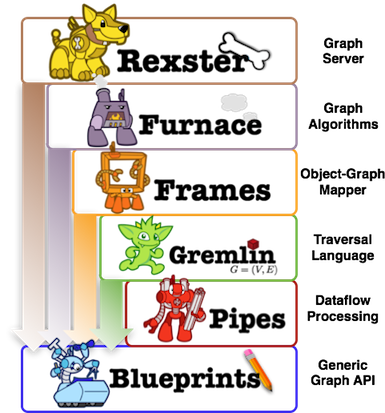
\includegraphics{rexster-system-arch}
    \caption{Stos technologiczny \emph{Tinkerpop}}
    \label{fig:tinkerpopStack}
\end{figure}

Biblioteka \emph{Blueprints} jest podstawą dla innych projektów, wspólnie tworzących stos technologiczny \emph{Tinkerpop} (rys.~\ref{fig:tinkerpopStack}):

\begin{itemize}
\item \emph{Pipes}: framework przepływu danych, umożliwiający dzielenie, łączenie, filtrowanie i transformację danych z wejścia do wyjścia,
\item \emph{Gremlin}: język trawersowania grafów bazujący na języku Groovy, pozwalający na tworzenie zapytań grafowych, analizę i manipulację danymi,
\item \emph{Frames}: biblioteka realizująca mapowanie obiektowo-grafowe, umożliwiająca tworzenie aplikacji w kontekście obiektów domenowych wraz z ich powiązaniami, a nie krawędzi i wierzchołków,
\item \emph{Furnace}: zestaw implementacji standardowych algorytmów analizy grafów,
\item \emph{Rexster}: serwer grafowy, udpstępniający grafy \emph{Blueprints} poprzez \emph{REST} oraz protokół \emph{RexPro}.
\end{itemize}



%---------------------------------------------------------------------------

\section{Wersjonowanie danych grafowych}
\label{sec:werjsonowanieDanychGrafowych}

\subsubsection{\emph{Git}}
\label{sec:git}

Kontrolę wersji danych grafowych można oprzeć o istniejący, sprawdzony system kontroli wersji - np. Git. Zapisane w postaci tekstowej (np. GraphML, GraphSON) snapshoty grafu można łatwo porównywać. Problem pojawia się natomiast, gdy chcemy przeszukać dane historyczne - konieczne jest wtedy odtworzenie grafu z pliku.

\subsubsection{\emph{Antiquity}}
\label{sec:antiquity}

\emph{Antiquity} - wersjonowany graf dla \emph{Tinkerpop Blueprints}, umożliwia pobranie z bazy historycznych wersji wierzchołków oraz krawędzi. Przynależność obiektu do danej wersji jest określana przez właściwości - minimalny i minimalny numer wersji grafu dla której dany obiekt jest aktualny. Wersja grafu jest inkrementowana przy każdej zmianie grafu lub przy każdej transakcji.

\subsubsection{\emph{FluxGraph}}
\label{sec:fluxGraph}

\emph{FluxGraph}\footnote{\url{https://github.com/datablend/fluxgraph}} to implementacja \emph{Tinkerpop Blueprints} dla bazy danych \emph{Datomic}. Baza ta przechowuje dane jako niezmienne (ang. \emph{immutable}) obiekty, opisane datą. \emph{FluxGraph} daje możliwość porównania grafu pomiędzy dwiema datami oraz porównania ze sobą dwóch obiektów. Dla każdego wierzchołka i krawędzi można także pobrać jego poprzednią i następną wersję. Datomic pod spodem może korzystać z baz relacyjnych, \emph{DynamoDB}, \emph{Riak}, \emph{Cassandra}, \emph{Couchbase}.

\subsubsection{Zapisywanie różnic pomiędzy zmianami}
\label{sec:roznice}

Rozwiązanie zaproponowane w \cite{journals/corr/abs-1302-5549}

\subsubsection{Graf historyczny o odmiennej strukturze}
\label{sec:castelltort}

W artykule \cite{conf/icdim/CastelltortL13} zaproponowano obiecującą metodę kontroli wersji danych grafowych, która zakłada nieinwazyjność - graf historyczny jest niezależny od danych źródłowych i może posiadać odmienną strukturę - np. wszystkie obiekty (także krawędzie) są zapisywane w grafie historycznym jako wierzchołki.


%\begin{figure}[htbp]
%    \centering
%    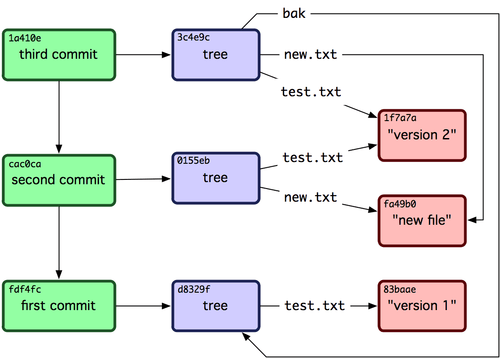
\includegraphics[width=0.8\textwidth]{git_tree}
%    \caption{Schemat bazy \emph{Git}}
%    \label{fig:gitTree}
%\end{figure}



%\chapter{Koncepcja rozwiązania i wymagania}
\label{cha:koncepcja}

W rozdziale tym zdefiniowano wymagania względem docelowego systemu oraz ogólną koncepcję rozwiązania.

%---------------------------------------------------------------------------

\section{Wymagania funkcjonalne}
\label{sec:wymaganiaFunkcjonalne}

\begin{itemize}
\renewcommand{\labelitemi}{$\bullet$}
  \item Tworzenie wersjonowanego grafu (\emph{init})
  \item Konwersja istniejącego grafu na graf wersjonowany (\emph{init} + \emph{add} + \emph{commit})
  \item Pobranie wersjonowanego grafu z serwera (\emph{clone})
  \item Pobranie najnowszych zmian z serwera (\emph{fetch})
  \item Scalenie zmian (\emph{merge})
  \item Uaktualnienie danych do najnowszej wersji z serwera (pobranie zmian i automatyczne scalenie) (\emph{pull})
  \item Zapisanie bieżącego stanu grafu jako nowej wersji (\emph{add} + \emph{commit})
  \item Tworzenie gałęzi (\emph{branch}), przełączanie się pomiędzy gałęziami (\emph{checkout})
  \item Wyświetlenie szczegółów zmian, porównania pomiędzy dwoma zmianami (\emph{diff})
  \item Wysłanie zmian na serwer (\emph{push})
  \item Wycofanie zmian (\emph{revert})
  \item Przywrócenie wybranych danych do konkretnej wersji (\emph{checkout})
\end{itemize}

%---------------------------------------------------------------------------

\section{Wymagania niefunkcjonalne}
\label{sec:wymaganiaNiefunkcjonalne}

\begin{itemize}
\renewcommand{\labelitemi}{$\bullet$}
\renewcommand{\labelitemii}{$\bullet$}
  \item Wymagania systemowe i technologiczne
  \begin{itemize}
     \item Interfejs konsolowy
     \item API  udostępniające pełną funkcjonalność (Java, Scala)
     \item Możliwość wykorzystania różnych grafowych baz danych
     \item System rozproszony (wzorowany na \emph{Git})
  \end{itemize}
\end{itemize}



%---------------------------------------------------------------------------

\section{Koncepcja rozwiązania}
\label{sec:koncepcjaRozwiazania}

Zakłada się, że wszystkie dane, konieczne do wersjonowania grafu, będą przechowywane w bazie danych, która podlega wersjonowaniu. Mechanizm wersjonowania korzystał będzie z interfejsu grafowego \emph{Tinkerpop Blueprints}, co umożliwi skorzystanie z różnych systemów bazodanowych. Obecnie dostępne są implementacje dla: TinkerGraph, Neo4J, Sail, OrientDB, Dex, Accumulo, ArangoDB, Bitsy, FluxGraph, FoundationDB, InfiniteGraph, MongoDB, Oracle NoSQL, Titan.

\begin{description}
\item[Koncepcja 1] Działanie zbliżone do \emph{Git}, czyli zmiany zostają poddane kontroli wersji w wyniku wywołania funkcji \emph{commit}. Użytkownik wprowadza dowolne zmiany w bazie danych i w wybranym przez siebie momencie tworzy \emph{snapshota}. Zaletą takiego rozwiązania jest przejrzysta historia zmian i mniejszy narzut na rozmiar bazy danych. Wadą jest to, że historia zmian nie jest zapisywana automatycznie. Schemat wersjonowanego grafu będzie przypomniał ten z rysunku~\ref{fig:gitTree}
\item[Koncepcja 2] Każda operacja na danych (dodanie/usunięcie wierzchołka/krawędzi lub grupy wierzchołków/krawędzi, edycja właściwości wierzchołka/krawędzi) prowadzi do powstania nowszej wersji grafu (generowany jest nowy numer wersji i nadawany jest on nowym wierzchołkom/krawędziom lub znacznikom usunięcia wierzchołka/krawędzi). Historia zapisywana jest więc automatycznie, lecz jest mniej przejrzysta (duża ziarnistość \emph{commitów}), wymaga też zapisania większej ilości informacji w bazie danych. Według tej koncepcji działa wersjonowany graf \emph{Antiquity}\footnote{\url{https://github.com/asaf/antiquity}}, będący pluginem do \emph{Blueprints}, nie zostanie on jednak wykorzystany z uwagi na zbyt ubogą dokumentację (brak informacji w jaki sposób dane o wersjach przechowywane są wewnętrznie, nie ma więc pewności, że jest to rozwiązanie optymalne) oraz zbyt małą funkcjonalność (nie przechowuje autorów zmian).
\end{description}




% itd.
% \appendix
% \include{dodatekA}
% \include{dodatekB}
% itd.


\nocite{*}
\bibliographystyle{alpha}
\bibliography{bibliografia}

%\begin{thebibliography}{1}
%
%\bibitem{Dil00}
%A.~Diller.
%\newblock {\em LaTeX wiersz po wierszu}.
%\newblock Wydawnictwo Helion, Gliwice, 2000.
%
%\bibitem{Lam92}
%L.~Lamport.
%\newblock {\em LaTeX system przygotowywania dokumentów}.
%\newblock Wydawnictwo Ariel, Krakow, 1992.
%
%\bibitem{Alvis2011}
%M.~Szpyrka.
%\newblock {\em {On Line Alvis Manual}}.
%\newblock AGH University of Science and Technology, 2011.cccccc
%\newblock \\\texttt{http://fm.ia.agh.edu.pl/alvis:manual}.
%
%\end{thebibliography}

\end{document}
